% !Mode:: "TeX:UTF-8"
% !TEX program  = xelatex
\documentclass{sdureport}

% no head line or foot line
%\pagestyle{empty}

% just for filling a few pages
\usepackage{blindtext}

% initialize the variable texts
\sduCollege{计算机科学与技术}
\sduCourse{模式识别与机器学习}
\sduSdudentId{202012345678}
\sduName{李阳}
\sduClass{智能19}
\sduExperimentalTopics{决策树}
\sduExexperimentalHours{4h}
\sduDate{\today}

\begin{document}
\begin{sduDocument}	

	\section{硬件环境}
	\begin{itemize}[leftmargin=1em] 
		\item Lenovo Legion Y7000P 2020H(16GB DDR4), Intel Core i7-10750H
		\item Windows 10, Chinese version
	\end{itemize}

	\section{软件环境}
	\begin{itemize}[leftmargin=1em] 
		\item Visual Studio Code 1.55.2
	\end{itemize}
	
	\section{实验目的}
	
	\begin{itemize}[leftmargin=1em]
		\item 利用已有的数据集 wine data 实现决策树
		\item 利用k=10折交叉验证评估决策树
		\item 决策树可视化
	\end{itemize}

	\section{实验记录}
	
	\subsection{C4.5决策树}

	C4.5算法是用于生成决策树的一种经典算法,是ID3算法的一种延伸和优化。

	C4.5算法对ID3算法主要做了一下几点改进:
	\begin{enumerate}
		\item 通过信息增益率选择分裂属性,克服了ID3算法中通过信息增益倾向于选择拥有多个属性值的属性作为分裂属性的不足。
		\item 能够处理离散型和连续型的属性类型,即将连续型的属性进行离散化处理。
		\item 构造决策树之后进行剪枝操作。
		\item 能够处理具有缺失属性值的训练数据。
	\end{enumerate}

	通过读取 ex6Data.csv 的数据,可以发现11个特征均为连续型属性,且整体数据量庞大需要剪枝操作,因此本次实验选用C4.5决策树是十分合适的。

	\subsubsection{分裂属性的选择:信息增益率}

	分裂属性选择的评判标准是决策树算法之间的根本区别。区别于ID3算法通过信息增益选择分裂属性,C4.5算法通过信息增益率选择分裂属性。

	设$D$是类标记元组训练集,类标号属性具有$m$个不同值,$m$个不同类$C^i,\quad i=1,2,\cdots,m$,$C^i_D$是$D$中$C^i$类的元组的集合,$|D|$和$|C^i_D|$分别是$D$和$C^i_D$中的元组个数。

	对于一个数据集合$D$,其信息熵为\[Info(D)=-\sum_{i=1}^{m}p_i\log_2(p_i)\]

	现在假定按照属性$A$划分$D$中的元组,且属性$A$将$D$划分成$v$个不同的类。在该划分之后,新的信息熵为\[Info_A(D)=\sum_{j=1}^{v}\frac{|D_j|}{|D|}\times Info(D_j)\]

	由此得到按照属性$A$划分$D$所获得的信息增益为原熵与新熵之差\[Gain(A)=Info(D)-Info_A(D)\]
	
	信息增益率使用“分裂信息”值将信息增益规范化。分类信息类似于$Info(D)$,定义为\[SplitInfo_A(D)=-\sum_{j=1}^{v}\frac{|D_j|}{|D|}\times \log_2(\frac{|D_j|}{|D|})\]

	由此定义信息增益率为\[GainRatio(A)=\frac{Gain(A)}{SplitInfo(A)}\]

	通过上述计算,最终选择具有最大信息增益率的属性作为分裂属性。

	\begin{figure}[H]
		\subfigure[熵]{
			\label{L1}
			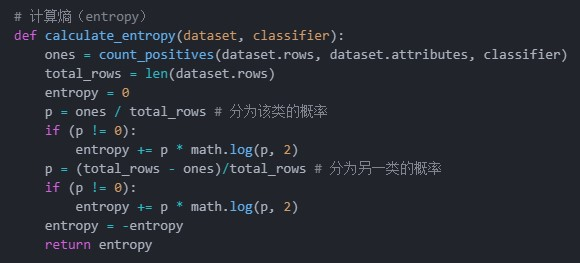
\includegraphics[width=0.45\textwidth]{image/5.7.1.jpg}}
		\subfigure[信息增益]{
			\label{b1}
			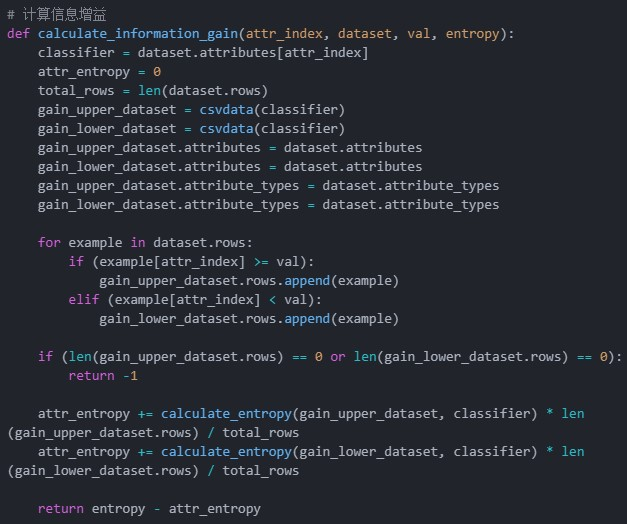
\includegraphics[width=0.45\textwidth]{image/5.7.2.jpg}}
		\caption{信息增益率}
	\end{figure}

	\subsubsection{连续型属性的离散化处理}

	当属性类型为离散型,无须对数据进行离散化处理;当属性类型为连续型,则需要对数据进行离散化处理。

	C4.5算法针对连续属性的离散化处理的核心思想是:
	\begin{enumerate}
		\item 将属性$A$的$N$个属性值按照升序排列,得到属性$A$的属性值取值序列$x_1^A,x_2^A,\cdots,x_N^A$。
		\item 在序列$x_1^A,x_2^A,\cdots,x_N^A$中共有$N-1$种二分方法,产生$N-1$种分隔阈值,对于第$i$种二分方法,其阈值$\theta_i=\frac{x_i^A+x_{i+1}^A}{2}$,它将该节点上的数据集划分为$2$个子数据集$x_1^A,x_2^A,\cdots,x_i^A$和$x_{i+1}^A,x_{i+2}^A,\cdots,x_N^A$。
		\item 计算每种划分方法对应的信息增益,选取信息增益最大的划分方法的阈值作为属性$A$二分的阈值。
	\end{enumerate}

	\begin{figure}[H]
		\begin{center}
		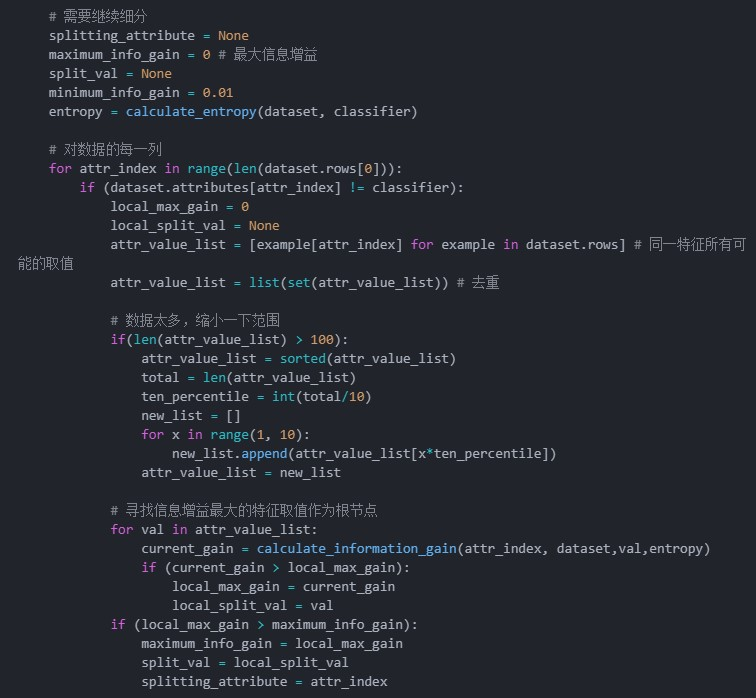
\includegraphics[width=0.5\textwidth]{image/5.7.3.jpg}
		\end{center}
		\caption{离散化处理}
	\end{figure}
	
	\subsubsection{剪枝}

	由于决策树的建立完全是依赖于训练样本,因此该决策树对训练样本能够产生完美的拟合效果。但这样的决策树对于测试样本来说过于庞大而复杂,可能产生较高的分类错误率。这种现象就称为过拟合。
	
	因此需要将复杂的决策树进行简化,即去掉一些节点解决过拟合问题,这个过程称为剪枝。

	剪枝方法分为预剪枝和后剪枝两大类。
	
	预剪枝是在构建决策树的过程中,提前终止决策树的生长,从而避免过多的节点产生。预剪枝方法虽然简单但实用性不强,因为很难精确的判断何时终止树的生长。
	
	后剪枝是在决策树构建完成之后,对那些置信度不达标的节点子树用叶子结点代替,该叶子结点的类标号用该节点子树中频率最高的类标记。

	\begin{figure}[H]
		\begin{center}
		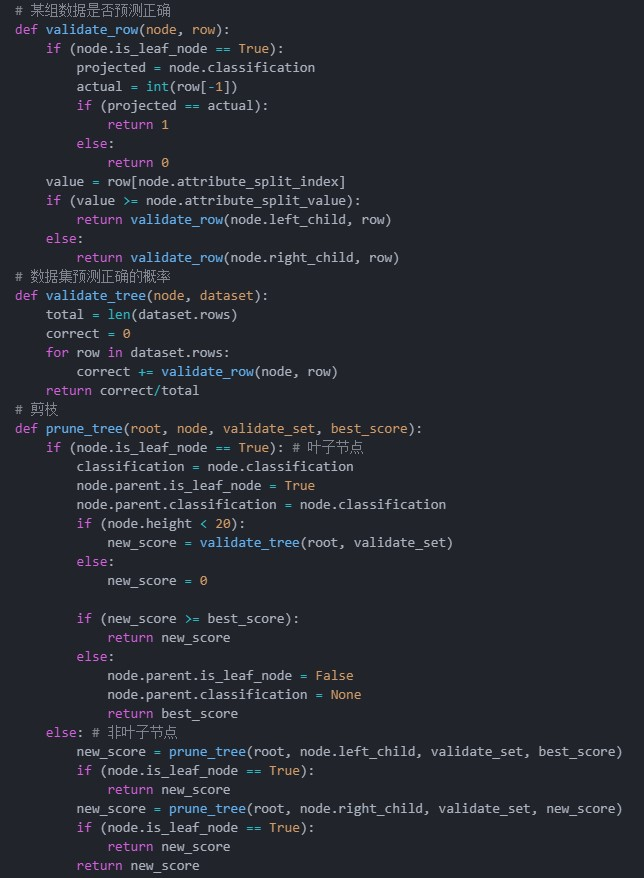
\includegraphics[width=0.5\textwidth]{image/5.7.4.jpg}
		\end{center}
		\caption{后剪枝操作}
	\end{figure}

	\subsection{K折交叉验证}

	将训练集数据划分为$K$部分,利用其中的$K-1$份做为训练,剩余的一份作为测试,最后取平均测试误差做为泛化误差。

	K折交叉验证利用了无重复抽样技术的好处:每次迭代过程中每个样本点只有一次被划入训练集或测试集的机会。

	\begin{figure}[H]
		\begin{center}
		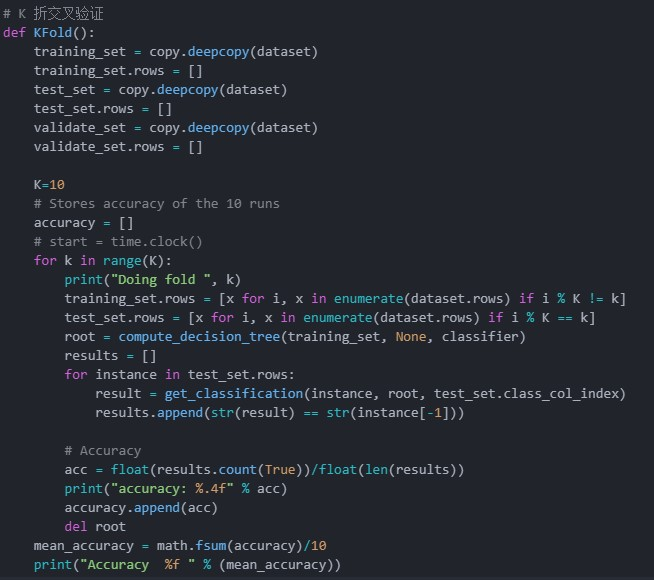
\includegraphics[width=0.4\textwidth]{image/5.7.5.jpg}
		\end{center}
		\caption{K折交叉验证函数}
	\end{figure}

	\subsection{可视化决策树}

	由于我个人的决策树实现不能像sklearn库中的那么完美,最终成型的决策树过于庞大,但是经过10折交叉验证,准确率有83\%

	\begin{figure}[H]
		\begin{center}
		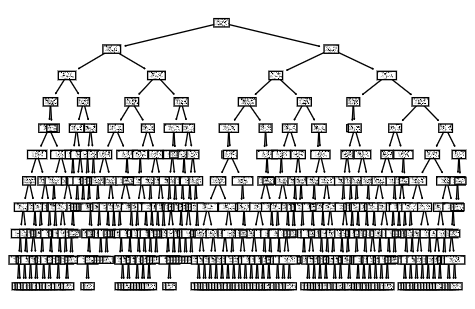
\includegraphics[width=0.5\textwidth]{image/1.png}
		\end{center}
		\caption{可视化决策树}
	\end{figure}

	\section{结论与分析}

	C4.5决策树算法优缺点分析\\

	\textbf{优点:}
	\begin{enumerate}
		\item 通过信息增益率选择分裂属性,克服了ID3算法中通过信息增益倾向于选择拥有多个属性值的属性作为分裂属性的不足。
		\item 能够处理离散型和连续型的属性类型,即将连续型的属性进行离散化处理。
		\item 构造决策树之后进行剪枝操作。
		\item 能够处理具有缺失属性值的训练数据
	\end{enumerate}

	\textbf{缺点:}
	\begin{enumerate}
		\item 算法的计算效率较低,特别是针对含有连续属性值的训练样本时表现的尤为突出。
		\item 算法在选择分裂属性时没有考虑到条件属性间的相关性,只计算数据集中每一个条件属性与决策属性之间的期望信息,有可能影响到属性选择的正确性。
	\end{enumerate}

\end{sduDocument}

\end{document}
